\documentclass[../Main.tex]{subfiles}

\begin{document}
\author{Internal Resistance} %use author for title of lesson
\date{Year 1 Topic 15} %use date to refer to topic in main booklet

\section{Internal Resistance} %Section is the title of the lesson repeated, ready for the main contents page.

\begin{frame}{Electromotive Force}
    Up to now we have said that the emf of a battery is the total voltage provided to a circuit. While this is generally true, it is not strictly what the emf of a battery is...
    \pause
    \begin{block}{emf}
    The emf of a battery is the potential difference across the battery \emph{when no current flows}. 
    \end{block}
\end{frame}

\begin{frame}{Internal Resistance}
     Batteries aren't perfect. There are chemicals in them that will restrict the flow of current leaving the battery. It is from this that we get internal resistance. 
    \begin{figure}
        \centering
        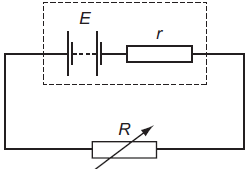
\includegraphics[height=4cm]{Electricity_Images/internal_resistance_circuit.png}
    \end{figure}
    This results in charge carriers having less energy than they would, in which case we have a \emph{lost voltage}.
    This means the rest of the circuit receives less voltage than it would do if there were no internal resistance.
\end{frame}

\begin{frame}{Formula Time!}
    There is a formula for internal resistance:
    
    \begin{equation*}
        \varepsilon = Ir + IR = I(r+R)
    \end{equation*}
    where I is the current flowing, r is the internal resistance and R is the total load resistance. \pause \newline
    \newline
    We can see that ``IR" is just the actual p.d. supplied to the rest of the circuit (also known as the terminal p.d.) and ``$V_{lost}=Ir$". Hence, we can say:
    \begin{equation*}
        \mbox{emf }= \mbox{lost voltage (Ir) + terminal voltage}
    \end{equation*}
    
    \begin{exampleblock}{Example}
    A battery has an emf of 9V, with a 100 $\Omega$ load. The current is 45mA. Calculate the internal resistance of the battery. \pause
    --100$\Omega$
    \end{exampleblock}
\end{frame}

\begin{frame}{Is it useful?}
    It can be useful for a power supply to have an internal resistance, or more useful to have none. 
    \newline \newline
    In an ideal world, no battery would have internal resistance - you would not want your phone battery to waste its charge overcoming its own internal resistance. But it also means that we can have a large current to charge it quickly and lose less energy.
    \pause
    \newline \newline
    A large internal resistance means we could have large voltage, but relatively little current flowing, for example a lab power supply would deliver a lower current if you were to complete a circuit using your body, making it safer*
    \pause
    \begin{block}{Remember these!}
    There are other examples -- but these are some generally good ones to know. And you could be asked about these in an exam!
    \end{block}
    {\tiny *disclaimer - while it is \emph{safer}, do not complete any circuits using yourself as it can still seriously injure (or even kill) you!}
\end{frame}

\begin{frame}{Your turn!}
    Go to Kerboodle page 181 for the internal resistance summary questions -- you may skip Q3c unless you want to have a go at it, thinking back to GCSE Science - as we are doing power in a future lesson.
\end{frame}

\begin{frame}{Internal Resistance Graphically}
Suppose we had an V-I graph, with V on the y-axis and I on the x-axis. We could plot the terminal p.d and current in a circuit, supposing we couldn't neglect internal resistance. First we need our equation in the form $y=mx+c$:

\begin{equation*}
    \epsilon = Ir + V \mbox{ becomes } V=\epsilon - Ir
\end{equation*}
In this rearrangement, what would the gradient ``m" and the y-intercept ``+c" be? \pause

\begin{block}{Key points of the graph:}
For a battery with internal resistance, the gradient of a V-I graph is -r, and the y-intercept is the emf of the battery.
\end{block}

\end{frame}

\end{document}